%% SDR Testbed System Requirements Specification
%% Copyright (C) 2019 Libre Space Foundation
%%
%% This work is licensed under a
%% Creative Commons Attribution-ShareAlike 4.0 International License.
%%
%% You should have received a copy of the license along with this
%% work.  If not, see <http://creativecommons.org/licenses/by-sa/4.0/>.

\documentclass[english,titlepage,a4paper]{report}

\usepackage[utf8]{inputenc}
\usepackage[T1]{fontenc}
\usepackage[english]{babel}
\usepackage{color}
\usepackage{float}
\usepackage[hidelinks]{hyperref}
\usepackage{tikz}
\usetikzlibrary{arrows,positioning,fit}
\usepackage[toc,acronyms,section]{glossaries}
\usepackage{textcomp}

\newglossarystyle{definitions}{
  \glossarystyle{long}
  \renewenvironment{theglossary}{
    \begin{longtable}{
        p{3cm}
        p{\glsdescwidth}
      }
  }{
    \end{longtable}
  }
}
\newglossary*{definitions}{Definitions}

\newglossarystyle{references}{
  \glossarystyle{long}
  \renewenvironment{theglossary}{
    \begin{longtable}{
        p{3cm}
        p{\glsdescwidth}
      }
  }{
    \end{longtable}
  }
}
\newglossary*{references}{References}
\makeglossaries

%% definitions glossary
\newglossaryentry{SDR Testbed}{
  type=definitions,
  name=SDR Testbed,
  description={Software Defined Radio Testbed; the system specified in this document}
}
\newglossaryentry{experiment}{
  type=definitions,
  name=experiment,
  description={The procedure as a whole of validating \gls{SDR application} and technologies}
}
\newglossaryentry{job}{
  type=definitions,
  name=job,
  description={A set of actions queue to be executed on an automation server}
}
\newglossaryentry{scenario}{
  type=definitions,
  name=scenario,
  description={A set of ordered test cases for validating an \gls{SDR application}}
}
\newglossaryentry{SDR development platform}{
  type=definitions,
  name=SDR development platform,
  description={A development platform which provides toolkits for implementing software defined radios}
}
\newglossaryentry{SDR application}{
  type=definitions,
  name=SDR application,
  description={An application implemented using an \gls{SDR development platform}}
}

%% references glossary
\newglossaryentry{Robot Framework}{
  type=references,
  name=\href{https://robotframework.org/}{Robot Framework},
  description={A Python-based automation framework}
}
\newglossaryentry{VISA}{
  type=references,
  name=\href{https://en.wikipedia.org/wiki/Virtual\_instrument\_software\_architecture}{VISA},
  description={Virtual Instrument Software Architecture}
}
\newglossaryentry{HDF5}{
  type=references,
  name=\href{https://www.hdfgroup.org/solutions/hdf5/}{HDF5},
  description={Hierarchical Data Format, version 5}
}
\newglossaryentry{RFC2119}{
  type=references,
  name=\href{https://www.ietf.org/rfc/rfc2119.txt}{RFC2119},
  description={Key words for use in RFCs to Indicate Requirement Levels}
}
\newglossaryentry{Linux}{
  type=references,
  name=\href{https://www.linux.org/}{Linux},
  description={A Unix-like operating system}
}
\newglossaryentry{CentOS}{
  type=references,
  name=\href{https://www.centos.org/}{CentOS},
  description={An enterprise-class \gls{Linux} distribution}
}
\newglossaryentry{Git}{
  type=references,
  name=\href{https://git-scm.com/}{Git},
  description={A distributed version-control system}
}
\newglossaryentry{Git LFS}{
  type=references,
  name=\href{https://git-lfs.github.com/}{Git LFS},
  description={An open source \gls{Git} extension for versioning large files}
}
\newglossaryentry{GitLab}{
  type=references,
  name=\href{https://gitlab.com/}{GitLab},
  description={A web-based \gls{Git}-repository manager}
}
\newglossaryentry{GNU Radio}{
  type=references,
  name=\href{https://www.gnuradio.org/}{GNU Radio},
  description={An \gls{SDR development platform}}
}
\newglossaryentry{Pothos SDR}{
  type=references,
  name=\href{https://github.com/pothosware/PothosSDR}{Pothos SDR},
  description={An \gls{SDR development platform}}
}
\newglossaryentry{SCPI}{
  type=references,
  name=\href{https://en.wikipedia.org/wiki/Standard_Commands_for_Programmable_Instruments}{SCPI},
  description={Standard Commands for Programmable Instruments}
}
\newglossaryentry{PlutoSDR}{
  type=references,
  name=\href{https://www.analog.com/en/design-center/evaluation-hardware-and-software/evaluation-boards-kits/adalm-pluto.html}{PlutoSDR},
  description={An \acrshort{SDR} device}
}
\newglossaryentry{Airspy Mini}{
  type=references,
  name=\href{https://airspy.com/airspy-mini/}{Airspy Mini},
  description={An \acrshort{SDR} device}
}
\newglossaryentry{SDRPlay RSPduo}{
  type=references,
  name=\href{https://www.sdrplay.com/rspduo/}{SDRPlay RSPduo},
  description={An \acrshort{SDR} device}
}
\newglossaryentry{LimeSDR Mini}{
  type=references,
  name=\href{https://limemicro.com/products/boards/limesdr-mini/}{LimeSDR Mini},
  description={An \acrshort{SDR} device}
}
\newglossaryentry{bladeRF 2.0 micro}{
  type=references,
  name=\href{https://www.nuand.com/bladerf-2-0-micro/}{bladeRF 2.0 micro},
  description={An \acrshort{SDR} device}
}
\newglossaryentry{USRP B210}{
  type=references,
  name=\href{http://www.ettus.com/all-products/ub210-kit/}{USRP B210},
  description={An \acrshort{SDR} device}
}
\newglossaryentry{RTL-SDR v3}{
  type=references,
  name=\href{https://www.rtl-sdr.com/rtl-sdr-blog-v-3-dongles-user-guide/}{RTL-SDR v3},
  description={An \acrshort{SDR} device}
}
\newglossaryentry{RC-2SP4T-A18}{
  type=references,
  name=\href{https://www.minicircuits.com/WebStore/dashboard.html?model=RC-2SP4T-A18}{RC-2SP4T-A18},
  description={A dual programmable \acrshort{SP4T} \acrshort{RF} switch}
}
\newglossaryentry{RCDAT-6000-60}{
  type=references,
  name=\href{https://www.minicircuits.com/WebStore/dashboard.html?model=RCDAT-6000-60}{RCDAT-6000-60},
  description={A programmable attenuator}
}
\newglossaryentry{BW-S30W2+}{
  type=references,
  name=\href{https://www.minicircuits.com/WebStore/dashboard.html?model=BW-S30W2\%2B}{BW-S30W2+},
  description={A fixed attenuator}
}
\newglossaryentry{BW-S20W2+}{
  type=references,
  name=\href{https://www.minicircuits.com/WebStore/dashboard.html?model=BW-S20W2\%2B}{BW-S20W2+},
  description={A fixed attenuator}
}
\newglossaryentry{gr-leo}{
  type=references,
  name=\href{https://gitlab.com/librespacefoundation/gr-leo}{gr-leo},
  description={A \gls{GNU Radio} space telecommunication simulator}
}
\newglossaryentry{gr-soapy}{
  type=references,
  name=\href{https://gitlab.com/librespacefoundation/gr-soapy}{gr-soapy},
  description={A GNURadio wrapper for the SoapySDR library}
}
\newglossaryentry{Docker}{
  type=references,
  name=\href{https://www.docker.com/}{Docker},
  description={A container technology}
}

%% Acronyms
\newacronym{SDR}{SDR}{Software Defined Radio}
\newacronym{CPU}{CPU}{Central Processing Unit}
\newacronym{RAM}{RAM}{Random Access Memory}
\newacronym{USB}{USB}{Universal Serial Bus}
\newacronym{TX}{TX}{Radio transmission}
\newacronym{RX}{RX}{Radio reception}
\newacronym{COTS PC}{COTS PC}{Commercial Off-The-Shelf Personal Computer}
\newacronym{IP}{IP}{Internet Protocol}
\newacronym{PSU}{PSU}{Power Supply Unit}
\newacronym{RF}{RF}{Radio Frequency}
\newacronym{OS}{OS}{Operating System}
\newacronym{SP4T}{SP4T}{Single pole, quad throw}
\newacronym{API}{API}{Application Programming Interface}
\newacronym{ATDD}{ATDD}{Acceptance Test–Driven Development}
\newacronym{HIL}{HIL}{Hardware-In-the-Loop}
\newacronym{SSD}{SSD}{Solid-State Drive}
\newacronym{CI}{CI}{Continuous Integration}

%% Glossary
\newglossaryentry{Ethernet}{
  name=Ethernet,
  description={A computer networking technology}
}
\newglossaryentry{x86-64}{
  name=x86-64,
  description={A 64-bit computer architecture}
}
\newglossaryentry{CPU thread}{
  name={CPU thread},
  description={\acrshort{CPU} concurrent execution}
}
\newglossaryentry{I/Q data}{
  name={I/Q data},
  description={In-phase and quadrature components data}
}

%% requirements command
\newcommand{\requirement}[5]{
  \subsection{#2}
  #5

  \noindent
  \begin{tabular}{|l|p{9cm}|}
    \hline
    \textbf{ID} & #1 \\
    \hline
    \textbf{Name} & #2 \\
    \hline
    \textbf{Description} & #3 \\
    \hline
    \textbf{Rationale} & #4 \\
    \hline
  \end{tabular}
}

\title{
  System Requirements Specification \\
  \large Software Defined Radio Testbed
}
\author{Vasilis Tsiligiannis} 
\date{\today\\\textit{DRAFT}}

\begin{document}
\renewcommand*{\arraystretch}{2}
\maketitle
\tableofcontents


\chapter{Introduction}
\section{Purpose}

The purpose of this document is to identify and create a complete set of Software and Hardware Requirements Specifications for implementing a Software Defined Radio Testbed.
The analysis shall contain an architectural overview and high level design and requirements specification which will be the basis to bootstrap the development and integration process.
Such an analysis is necessary in order to provide implementers a clear view and understanding of the system under development as well as defining standard interfaces for users of the system.

\section{Conventions}

The key words "MUST", "MUST NOT", "REQUIRED", "SHALL", "SHALL NOT", "SHOULD", "SHOULD NOT", "RECOMMENDED", "MAY", and "OPTIONAL" in this document are to be interpreted as described in \gls{RFC2119}.
However, for readability, these words do not appear in all upper case letters in this specification.

\newpage
\printglossary[type=definitions,numberedsection,style=definitions,nonumberlist]

\section{Intended Audience}

The intended audience of this document are hardware and software developers who will implement the \gls{SDR Testbed} described.
It is assumed that the reader is familiar with Software Defined Radio systems and has knowledge of software engineering as well as IT systems in general.

\section{Scope}

The Software Defined Radio Testbed system described in this document plans to become an essential tool for the research and development of \acrshort{SDR}-based satellite communication systems.
This testbed will allow early experimentation and testing of new algorithms and configurations.
The implementation of an \gls{SDR Testbed} system will span from software and hardware development to integration of various \acrshort{SDR} toolchains and hardware components.

\newpage
\printglossary[type=references,numberedsection,style=references,nonumberlist]

\chapter{Description}
\section{System Functions}

This specification is based on high-level requirements which have been collected from various stakeholders.
The collection has been facilitated by the use of a requirements survey.
Based on the survey results and the resources allocated for the project, it is decided that the following high-level functions shall be supported:
\begin{itemize}
\item importing and exporting of data for input and output of \glspl{experiment}.
\item selection of various SDR device combinations.
\item single \acrshort{TX} and \acrshort{RX} paths.
\item selection of different attenuation levels between \acrshort{TX} and \acrshort{RX} devices.
\item telecommunication channel simulation.
\item first-come-first-served \gls{job} queuing.
\end{itemize}

Additionally, multiple iterations of design and implementation are planned which may further enhance or extend the above functions.
Note, that the above list is not exhaustive.
A more detailed list is provided later in chapter \ref{chapter_4}.

\begin{figure}[H]
  \centering
  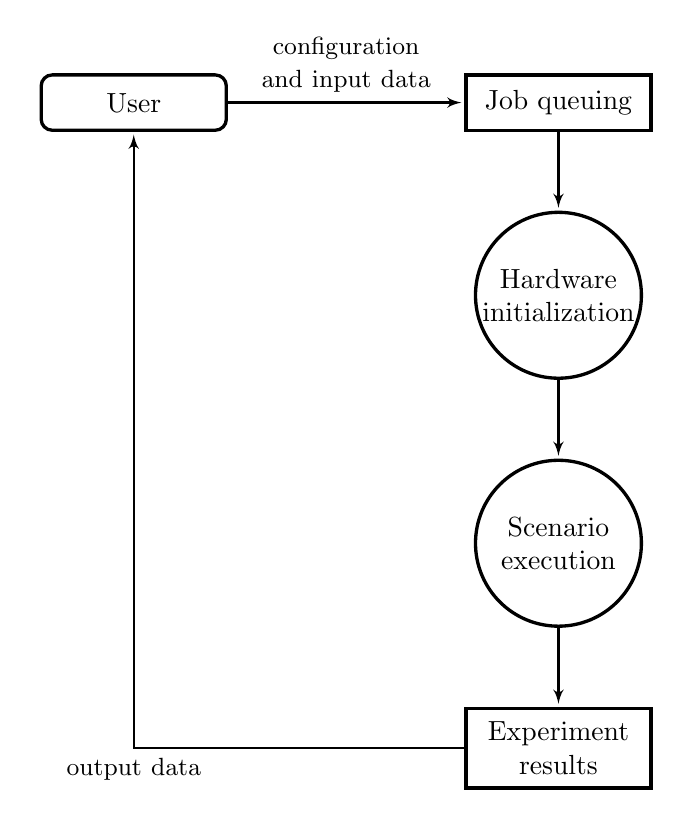
\begin{tikzpicture}[node distance=1cm,auto]
    \tikzset{
      circlenode/.style={circle,draw=black,very thick,inner sep=0em,minimum size=2cm,text width=2cm,text centered},
      rectroundnode/.style={rectangle,rounded corners,draw=black,very thick,inner sep=0.5em,minimum size=2em,text width=2cm,text centered},
      rectnode/.style={rectangle,draw=black,very thick,inner sep=0.5em,minimum size=2em,text width=2cm,text centered},
      arrowlabel/.style={text width=7em,text centered},
      arrow/.style={->,>=latex',shorten >=1pt,thick}
    }
    \node[rectroundnode](user){User};
    \node[rectnode,right=3cm of user](queue){Job queuing};
    \node[circlenode,below=of queue](initialization){Hardware initialization};
    \node[circlenode,below=of initialization](job){Scenario execution};
    \node[rectnode,below=of job](results){Experiment results};

    \draw[arrow](user.east) -- node[arrowlabel,above]{\small configuration and input data} (queue.west);
    \draw[arrow](queue.south) -- (initialization.north);
    \draw[arrow](initialization.south) -- (job.north);
    \draw[arrow](job.south) -- (results.north);
    \draw[arrow](results.west) -| node[arrowlabel,below]{\small output data} (user.south);
  \end{tikzpicture}
  \medskip
  \caption{Basic experiment flow}
  \label{basic flow}
\end{figure}

Figure \ref{basic flow} shows the very basic \gls{experiment} flow, based on the high-level functions.
The user submits the \gls{SDR Testbed} configuration as well as \gls{experiment} input data.
A \gls{job} queuing mechanism queues the \gls{job} for the user.
Once the \gls{job} is picked up, the hardware is initialized, based on the configuration parameters.
The \gls{experiment} \gls{scenario} is executed using the input data provided.
As a final step, the result of the \gls{experiment} is output and becomes available to the user.

\section{System Perspective}

\begin{figure}[H]
  \centering
  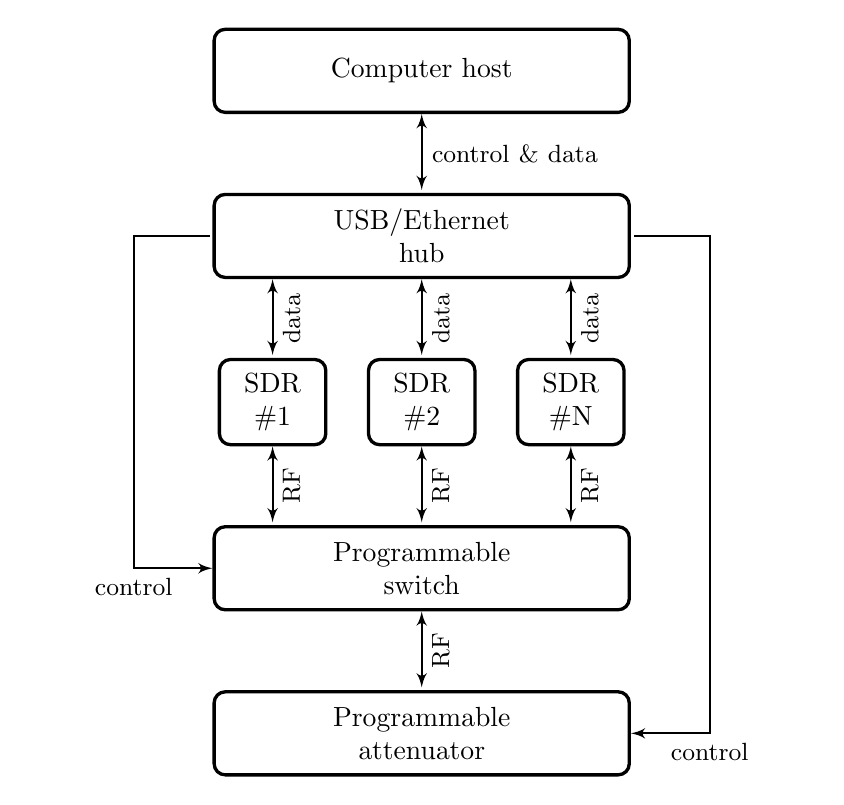
\begin{tikzpicture}[node distance=1cm,auto]
    \tikzset{
      rectroundnode/.style={rectangle,rounded corners,draw=black,very thick,inner sep=0.5em,minimum height=3em,text width=2.5cm,text centered},
      arrowlabel/.style={text width=7em},
      arrow/.style={<->,>=latex',shorten >=1pt,thick}
    }
    \node[rectroundnode,minimum width=15em](host){Computer host};
    \node[rectroundnode,below=of host,minimum width=15em](hub){USB/Ethernet hub};
    \node[rectroundnode,below=of hub,text width=1cm](sdr2){SDR \#2};
    \node[rectroundnode,left=0.5cm of sdr2,text width=1cm](sdr1){SDR \#1};
    \node[rectroundnode,right=0.5cm of sdr2,text width=1cm](sdrn){SDR \#N};
    \node[rectroundnode,below=of sdr2,minimum width=15em](progswitch){Programmable switch};
    \node[rectroundnode,below=of progswitch,minimum width=15em](progatt){Programmable attenuator};

    \draw[arrow](host.south) -- node[arrowlabel,right]{\small control \& data} (hub.north);
    \draw[arrow](hub.south) -- node[arrowlabel,right]{\rotatebox{90}{\small data}} (sdr2.north);
    \draw[arrow](hub.south -| sdr1.north) -- node[arrowlabel,right]{\rotatebox{90}{\small data}} (sdr1.north);
    \draw[arrow](hub.south -| sdrn.north) -- node[arrowlabel,right]{\rotatebox{90}{\small data}} (sdrn.north);
    \draw[arrow](sdr2.south) -- node[arrowlabel,right]{\rotatebox{90}{\small RF}} (progswitch.north);
    \draw[arrow](sdr1.south) -- node[arrowlabel,right]{\rotatebox{90}{\small RF}} (progswitch.north -| sdr1.south);
    \draw[arrow](sdrn.south) -- node[arrowlabel,right]{\rotatebox{90}{\small RF}} (progswitch.north -| sdrn.south);
    \draw[arrow](progswitch.south) -- node[arrowlabel,right]{\rotatebox{90}{\small RF}} (progatt.north);
    \draw[arrow,<-](progswitch.west) -| ++(-1cm,0) node[arrowlabel,below,text centered]{\small control} |- (hub.west);
    \draw[arrow,<-](progatt.east) -| ++(1cm,0) node[arrowlabel,below,text centered]{\small control} |- (hub.east);

  \end{tikzpicture}
  \medskip
  \caption{Example hardware block diagram}
  \label{hardware block diagram}
\end{figure}

The \gls{SDR Testbed} consists both of software and hardware components.
Figure \ref{hardware block diagram} shows an example high-level block diagram of the hardware components.
These components are:
\begin{itemize}
\item A computer host where the \gls{SDR Testbed} software is running.
\item A \acrshort{USB} or/and \gls{Ethernet} hub for the \acrshort{SDR} devices and programmable \acrshort{RF} components to connect with the host.
\item A set of \acrshort{SDR} devices.
\item A set of programmable \acrshort{RF} components (e.g. \acrshort{RF} switch, attenuators, etc.).
\item A set of fixed components (e.g. \acrshort{USB}, \gls{Ethernet}, \acrshort{RF} cables and connectors, fixed attenuators, etc.).
\end{itemize}

\noindent
\begin{figure}[H]
  \centering
  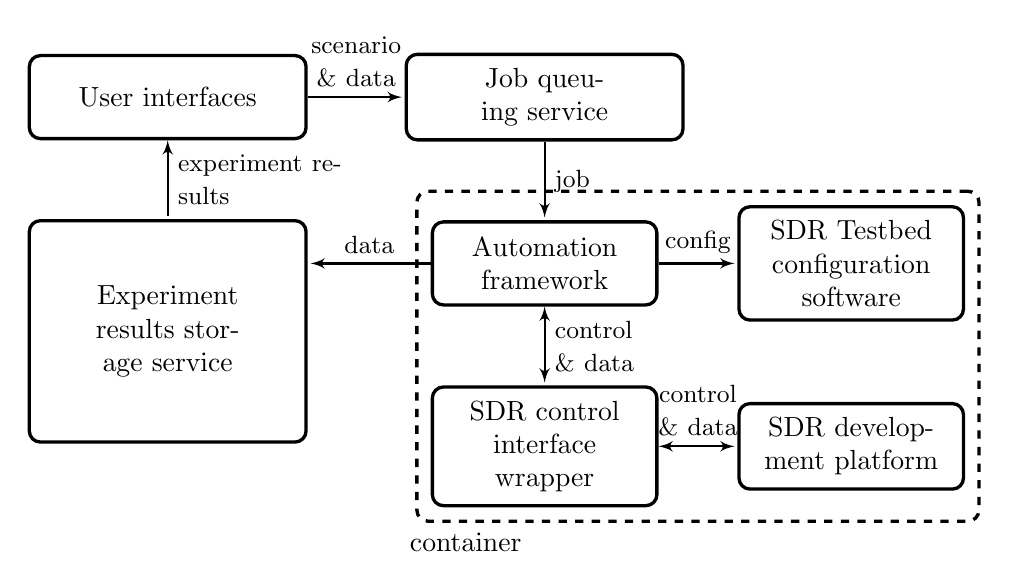
\begin{tikzpicture}[node distance=1cm,auto]
    \tikzset{
      rectroundnode/.style={rectangle,rounded corners,draw=black,very thick,inner sep=0.5em,minimum height=3em,text width=2.5cm,text centered},
      rectfit/.style={rounded corners,draw=black,very thick,inner sep=0.5em,minimum height=3em,text width=2.5cm,text centered},
      arrowlabel/.style={text width=7em},
      arrow/.style={<->,>=latex',shorten >=1pt,thick}
    }
    \node[rectroundnode,minimum width=10em](userinterface){User interfaces};
    \node[rectroundnode,right=3.5em of userinterface,minimum width=10em](jobserver){Job queuing service};
    \node[rectroundnode,below=of jobserver,minimum width=7em](automation){Automation framework};
    \node[rectroundnode,below=of automation,minimum width=7em](wrapper){SDR control interface wrapper};
    \node[rectroundnode,right=of automation,minimum width=7em](testbedconfig){SDR Testbed configuration software};
    \node[rectroundnode,right=of wrapper,minimum width=7em](sdrplatform){SDR development platform};
    \node[rectroundnode,minimum width=10em,minimum height=8em,below=of userinterface](storage){Experiment results storage service};
    \node[rectfit,fit=(automation)(testbedconfig)(wrapper),dashed,label={below left:container}](container){};

    \draw[arrow,->](userinterface.east) -- node[arrowlabel,above,text centered]{\small scenario \\ \& data} (jobserver.west);
    \draw[arrow,->](jobserver.south) -- node[arrowlabel,right]{\small job} (automation.north);
    \draw[arrow,->](automation.east) -- node[arrowlabel,above,text centered]{\small config} (testbedconfig.west);
    \draw[arrow](automation.south) -- node[arrowlabel,right]{\small control \\ \& data} (wrapper.north);
    \draw[arrow](wrapper.east) -- node[arrowlabel,above,text centered]{\small control \\ \& data} (sdrplatform.west);
    \draw[arrow,<-](userinterface.south) -- node[arrowlabel,right]{\small experiment results} (storage.north);
    \draw[arrow,->](automation.west) -- node[arrowlabel,above,text centered]{\small data} (storage.east |- automation.west);

  \end{tikzpicture}
  \medskip
  \caption{Example software block diagram}
  \label{software block diagram}
\end{figure}

Figure \ref{software block diagram} shows an example high-level block diagram of the software components.
These components are:
\begin{itemize}
\item Interfaces which the user uses to submit \glspl{scenario} and data and retrieve \gls{experiment} results.
\item A \gls{job} queuing service.
\item A container in which application are running.
\item An automation framework which executes the \gls{scenario} submitted by the user.
\item Software to configure the \gls{SDR Testbed}.
\item Software to act as a wrapper for controlling the \gls{SDR development platform}.
\item An \gls{SDR development platform} which the \gls{SDR application} is running.
\item A storage service where the \gls{experiment} results are stored.
\end{itemize}

As a whole, the \gls{SDR Testbed} shall be an independent and totally self-contained system and not part of a larger system.
Thus, no strict requirements for external interfaces are set.
Nevertheless, additional ready-made components not defined in this specification may be used to complete it.

\newpage
\section{Operating Environment}

The software operating environment shall be based, to the maximum extent possible, on free and open source software.
All software components of \gls{SDR Testbed} shall be running on \gls{Linux} \acrshort{OS}.
It is suggested that a modern enterprise grade \gls{Linux} distribution (e.g. \gls{CentOS}) should be used for this purpose.
The services and application shall be containerized to provide isolation and easier management.

The hardware operating environment can be based both on commercial and/or non-commercial hardware.
The testbed shall be developed for \gls{x86-64} hardware platform, either server or \acrshort{COTS PC}.
Nevertheless, provision has been made so that it should be possible to run on different architectures with minimal changes.
Most of the communication between hardware components shall be over \acrshort{USB} or \acrshort{IP} network.

\section{Design and Implementation Constraints}

The following design and implementation constraints will be present on the \gls{SDR Testbed}:
\begin{itemize}
\item \Glspl{job} will be queued and executed sequentially.
  The testbed can only handle a single \gls{experiment} at a time.
  Nevertheless, scaling-out will be possible i.e. by adding more \gls{SDR Testbed}s.
\item A limited number of \acrshort{SDR} devices will be supported.
  Hardware restrictions place a limit on the number of devices which can be supported.
  A fixed number of \acrshort{USB} and \gls{Ethernet} ports will be available on the system for connecting \acrshort{SDR} devices.
\item The duration of an \gls{experiment} will be limited.
  Since the \glspl{job} will be executed sequentially, a limit on the duration of \glspl{experiment} will be placed.
\end{itemize}

\section{Documentation}

The documentation shall consist of two parts:
\begin{itemize}
\item Users' documentation.
  This documentation shall be the manual on how to use the testbed from users' point of view.
\item Developers' documentation.
  This documentation shall be intended for developers on how to further extend or maintain the system.
\end{itemize}

\section{Assumption and Dependencies}

This system will be designed with the assumption that any \gls{experiment} will not exceed the performance limits of the hardware.
This includes \acrshort{CPU} power, \acrshort{RAM} available, storage space, etc. as well as electrical characteristics (e.g. \acrshort{PSU} or \acrshort{USB} power available).
See section \ref{performance requirements} for more details.


\chapter{External Interfaces}
\section{User Interfaces}

The entry point of the user to the \gls{SDR Testbed} shall be a \gls{Git} repository.
The user shall commit:
\begin{itemize}
\item the \gls{scenario} for an \gls{experiment}.
  This \gls{scenario} shall be written as a \gls{Robot Framework} Suite.
\item raw data to be fed to the \acrshort{SDR} devices.
  \gls{Git LFS} shall be used to commit raw \gls{I/Q data}.
\item configuration of the \gls{SDR Testbed} hardware.
  The configuration includes selection of the \acrshort{SDR} devices to be used and attenuation level.
\end{itemize}
The user shall push the commits to a remote \gls{Git} repository managed by \gls{GitLab}.
\gls{GitLab} \acrshort{CI} shall queue a \gls{job} to be executed to the computer host where the \acrshort{SDR} devices are attached.
After the execution and completion of the \gls{job}, the host shall upload the results to the server managing the \glspl{job}.
The user shall be able to view and download the results of the \gls{experiment} from the \gls{job} server.

\newpage
\section{Software Interfaces}

The \gls{SDR Testbed} shall have the following software interfaces:
\begin{itemize}
\item an \gls{SDR development platform}.
  \gls{GNU Radio} shall be the platform initially supported.
  Nevertheless, it shall be possible to support other platforms in the future (i.e. \gls{Pothos SDR}).
\item \gls{VISA} \acrshort{API} and instrument drivers.
  \gls{VISA} is a standard instrument control abstraction layer and shall be used to control the programmable \acrshort{RF} switches and attenuators.
\item an \acrshort{SDR} control and data interface.
  A new software interface shall be developed to abstract the control and data exchange towards the \gls{SDR application}.
  This interface shall act as a wrapper function with a purpose to allow realtime control of the \acrshort{SDR} during an \gls{experiment}.
\item an \gls{experiment} results file format interface.
  \gls{HDF5} file format shall be used to store some \gls{experiment} results.
  This interface shall be the library for supporting \gls{HDF5} storing.
\end{itemize}

\section{Hardware Interfaces}

The \gls{SDR Testbed} shall have the following hardware interfaces:
\begin{itemize}
\item \acrshort{USB} interfaces for connecting \acrshort{SDR} devices.
\item \gls{Ethernet} interfaces for connecting \acrshort{SDR} devices and programmable \acrshort{RF} switches and attenuators.
\item \acrshort{RF} interfaces for connecting \acrshort{SDR} devices with programmable switches and attenuators.
\end{itemize}

\section{Communication Interfaces}

The \gls{SDR Testbed} shall have the following communication interfaces:
\begin{itemize}
\item \gls{SCPI}.
  This interface shall be used to control the programmable \acrshort{RF} switch and attenuators.
\item \acrshort{SDR} control and data sockets.
  Separate network or Unix domain sockets shall be used for controlling and exchanging data with the \gls{SDR development platform}.
  These communication interface shall provide support for realtime control of the \gls{SDR application}.
\end{itemize}

\chapter{Requirements} \label{chapter_4}
\section{Functional Requirements}

\requirement{REQ.0001}{Availability of computer host USB ports}{
  The computer host shall have at least 4 x USB3.x and 2 x USB2.x ports.
}{
  Most of the \acrshort{SDR} devices interface via \acrshort{USB}.
  The computer host should have enough \acrshort{USB} ports to accommodate all available \acrshort{SDR} devices.
}{}
\requirement{REQ.0002}{Availability of computer host Ethernet}{
  The computer host shall have at least one 1000BASE‑T \gls{Ethernet} port.
}{
  Some \acrshort{SDR} devices interface via \gls{Ethernet}.
  In addition, programmable \acrshort{RF} switches and attenuators interface via \gls{Ethernet}, too.
  The computer host should have at least one \gls{Ethernet} port capable of transferring data with high enough throughput to support these devices.
}{}
\requirement{REQ.0003}{Network connectivity for multiple devices}{
  An 8-port managed 1000BASE-T \gls{Ethernet} switch shall be used to provide network connectivity with devices.
}{
  A network switch is required to connect all the devices communication via \gls{Ethernet}.
  The switch shall be manageable for easy configuration, monitoring and adaptation on existing networking infrastructures.
}{}
\requirement{REQ.0004}{PlutoSDR SDR device support}{
  The \gls{SDR Testbed} shall support \gls{PlutoSDR} \acrshort{SDR} device.
}{
  Based on the requirements survey, \gls{PlutoSDR} is one of the selected \acrshort{SDR} devices to be supported.
}{}
\requirement{REQ.0005}{Airspy Mini SDR device support}{
  The \gls{SDR Testbed} shall support \gls{Airspy Mini} \acrshort{SDR} device.
}{
  Based on the requirements survey, \gls{Airspy Mini} is one of the selected \acrshort{SDR} devices to be supported.
}{}
\requirement{REQ.0006}{SDRPlay RSPduo SDR device support}{
  The \gls{SDR Testbed} shall support \gls{SDRPlay RSPduo} \acrshort{SDR} device.
}{
  Based on the requirements survey, \gls{SDRPlay RSPduo} is one of the selected \acrshort{SDR} devices to be supported.
}{}
\requirement{REQ.0007}{LimeSDR Mini SDR device support}{
  The \gls{SDR Testbed} shall support \gls{LimeSDR Mini} \acrshort{SDR} device.
}{
  Based on the requirements survey, \gls{LimeSDR Mini} is one of the selected \acrshort{SDR} devices to be supported.
}{}
\requirement{REQ.0008}{bladeRF 2.0 micro SDR device support}{
  The \gls{SDR Testbed} shall support \gls{bladeRF 2.0 micro} \acrshort{SDR} device.
}{
  Based on the requirements survey, \gls{bladeRF 2.0 micro} is one of the selected \acrshort{SDR} devices to be supported.
}{}
\requirement{REQ.0009}{USRP B210 SDR device support}{
  The \gls{SDR Testbed} shall support \gls{USRP B210} \acrshort{SDR} device.
}{
  Based on the requirements survey, \gls{USRP B210} is one of the selected \acrshort{SDR} devices to be supported.
}{}
\requirement{REQ.0010}{RTL-SDR v3 SDR device support}{
  The \gls{SDR Testbed} shall support \gls{RTL-SDR v3} \acrshort{SDR} device.
}{
  Based on the requirements survey, \gls{RTL-SDR v3} is one of the selected \acrshort{SDR} devices to be supported.
}{}
\requirement{REQ.0011}{Programmable selection of SDR devices}{
  A pair of programmable \acrshort{SP4T} \acrshort{RF} switches shall be used to select \acrshort{RF} connections between \acrshort{SDR} devices.
  The \acrshort{RF} switch characteristics shall be:
  \begin{itemize}
  \item isolation: >=60dB
  \item reliability: >=10Mcycles
  \item insertion loss: <=1dB
  \end{itemize}
  A candidate \acrshort{RF} switch is the \gls{RC-2SP4T-A18} from Mini-Circuits.
  A single pair of \acrshort{SDR} devices shall be connected at any time.
  A total of 16 combinations of \acrshort{SDR} devices shall be supported.
  %%Figure XXX shows a connection diagram between the programmable RF switch and the SDR devices
}{
  For each \gls{experiment} a pair of \acrshort{SDR} devices need to be selected.
  These devices should be \acrshort{RF} connected programmably.
  A pair of \acrshort{SP4T} \acrshort{RF} switches shall be used to provide such connectivity.
}{}
\requirement{REQ.0012}{Programmable selection of attenuation levels}{
  The attenuation levels between the pair of \acrshort{SDR} devices shall be controlled programmably.
  A single programmable \acrshort{RF} attenuator shall be used for this purpose.
  The \acrshort{RF} attenuator characteristics shall be:
  \begin{itemize}
  \item range: 0dB to -60dB
  \item resolution: 0.25dB
  \item power rating: 20dBm
  \item \gls{Ethernet} control
  \end{itemize}
  A candidate device is the \gls{RCDAT-6000-60} from Mini-Circuits.
  %%Figure XXX shows a connection diagram between the programmable RF switch and the SDR devices
}{
  An \gls{experiment} can require variable attenuation conditions.
  The testbed shall accommodate such cases by using a programmable attenuator.
}{}
\requirement{REQ.0013}{Fixed attenuation between selected SDR devices}{
  There shall be a fixed \acrshort{RF} attenuation between the selected pair of \acrshort{SDR} devices.
  This attenuation shall be -60dBm.
  Some candidate devices are the \gls{BW-S30W2+} or \gls{BW-S20W2+} from Mini-Circuits.
}{
  A fixed attenuation is required to emulate free-space path loss conditions.
  Combined with the programmable attenuator, this shall give an attenuation range of -60db to -120dB.
}{}

\requirement{REQ.0014}{GNU Radio SDR development platform support}{
  \gls{GNU Radio} shall be used as the \gls{SDR development platform}.
}{
  \gls{GNU Radio} is the de facto standard for developing \gls{SDR application}s.
}{}
\requirement{REQ.0015}{gr-leo support}{
  \gls{gr-leo} support shall be included with \gls{GNU Radio}.
}{
  \gls{gr-leo} is a space telecommunication simulator.
  Channel simulation is an essential feature for an \gls{SDR Testbed} focusing on satellite communications.
}{}
\requirement{REQ.0016}{gr-soapy support}{
  \gls{gr-soapy} support shall be included with \gls{GNU Radio}.
}{
  \gls{gr-soapy} is an interface to SoapySDR for \gls{GNU Radio}.
  It provides a clean \acrshort{API} for configuring various \acrshort{SDR} devices.
}{}
\requirement{REQ.0017}{Configurability of RF switches and attenuators}{
  A utility shall be developed to configure and control the \gls{SDR Testbed} hardware.
  This utility shall be used to control:
  \begin{itemize}
  \item programmable \acrshort{RF} switches
  \item programmable \acrshort{RF} attenuators
  \end{itemize}
  This application shall utilize \gls{VISA} and \gls{SCPI} protocols.
  The communication with the devices shall be via \gls{Ethernet}.
}{
  Programmable switches and attenuators need to be configured before the start or during the \gls{experiment}.
  The testbed needs to support such a function.
}{}
\requirement{REQ.0018}{Abstraction interface to SDR application}{
  A wrapper application shall be developed to provide an abstraction layer (\acrshort{API}) for executing \gls{SDR application}s.
  The wrapper shall provide separate control and data sockets.
  The socket shall be network or Unix domain sockets.
  The control socket shall be used for controlling the \gls{SDR application}.
  The data socket shall be used to exchanging data.
}{
  A form of an \acrshort{API} is required for the \gls{SDR Testbed} to execute \gls{SDR application} in a consistent way.
  Additionally, the above interfaces will allow realtime control of the \gls{SDR application}.
}{}
\requirement{REQ.0019}{Use of Git for submitting scenario and data}{
  \gls{Git} shall be used to submit \glspl{scenario} and data for an \gls{experiment}.
  \Glspl{scenario}, in the form of \gls{Robot Framework} suites shall be committed to a repository.
  Bulk data shall be committed in \gls{Git LFS}.
}{
  \gls{Git} is a software version control system.
  By using \gls{Git} to store \glspl{scenario} and data, \acrshort{ATDD} and \acrshort{HIL} is possible.
}{}
\requirement{REQ.0020}{GitLab CI as a job service}{
  \gls{GitLab} and \gls{GitLab} \acrshort{CI} shall be used as a \gls{job} and \gls{experiment} results storage service.
  The computer host shall be running a \gls{GitLab} Runner.
  The runner shall be registered to \gls{GitLab}.
  It shall be configured as a \gls{Docker} executor.
  Parallel \gls{job} execution shall not be allowed.
  \Gls{experiment} results shall be upload as artifacts to \gls{GitLab}.
}{
  \gls{GitLab} \acrshort{CI} is a continuous integration and delivery service.
  Such a \acrshort{CI} service is required by \gls{SDR Testbed} for \gls{job} queuing and storage of \gls{experiment} results.
}{}
\requirement{REQ.0021}{Support of Robot Test Automation Framework}{
  \gls{Robot Framework} shall be used as an Automation Framework.
  A set of libraries shall be developed to extend the framework:
  \begin{itemize}
  \item Library for controlling the \gls{SDR Testbed} configuration utility.
  \item Library for handling all functions of the \acrshort{SDR} controller.
  \end{itemize}
  \Gls{experiment} \glspl{scenario} shall be written as \gls{Robot Framework} Suites.
}{
  An automation framework is required to execute elaborate \glspl{scenario}.
  \gls{Robot Framework} is an automation framework for acceptance testing, acceptance test driven development (\acrshort{ATDD}), and robotic process automation (RPA).
  The framework needs to be extended with \gls{SDR Testbed} specific functions.
}{}
\requirement{REQ.0022}{Storing of experiment results in Hierarchical Data Format}{
  It shall be possible to store \gls{experiment} results in \gls{HDF5}\textsuperscript{\textregistered} format.
}{
  HDF is a file format designed to store and organize large amounts of data.
  Testbed \gls{experiment} which generated large amounts of data or need to store metadata information can benefit by \gls{HDF5}\textsuperscript{\textregistered} support.
}{}
\requirement{REQ.0023}{Limitation of experiment running time}{
  The amount of time an \gls{experiment} can be running shall be limited.
  A timeout of 30 minutes shall be set for this purpose.
  After the time has elapsed, the execution of the \gls{experiment} shall be terminated and the resources shall be freed.
}{
  The \gls{SDR Testbed} has limited resources since the \glspl{job} are executed sequentially.
  A limit has to be set on the time an \gls{experiment} will be running so that the testbed can be available to other users.
}{}
\requirement{REQ.0024}{Limitation of experiment results size}{
  The amount of data an \gls{experiment} can produce shall be limited.
  The maximum data that an \gls{experiment} can output shall be set to 100MiB.
  Data that exceed the above limit shall not be uploaded to the storage service.
}{
  The \gls{SDR Testbed} and storage service has limited resources.
  A limit has to be set on the amount of data an \gls{experiment} can generate.
}{}
\requirement{REQ.0025}{Containerization of SDR Testbed applications}{
  The following \gls{SDR Testbed} application shall be containerized with \gls{Docker}:
  \begin{itemize}
  \item \gls{Robot Framework}
  \item \gls{SDR Testbed} configuration utility
  \item \gls{GNU Radio}
  \item \acrshort{SDR} controller
  \end{itemize}
  A single container shall be created which will contain all the above software.
}{
  Containerizing the \gls{SDR Testbed} applications provides isolation, a reproducible environment and easier management.
  It also allows the use of \gls{GitLab} Runner \gls{Docker} executors.
}{}

\section{Performance Requirements} \label{performance requirements}

\requirement{REQ.0101}{Dimensions of computer host RAM}{
  The computer host shall have at least 16GiB of available \acrshort{RAM}.
}{
  Some \gls{SDR application}s are very demanding to \acrshort{RAM}.
  The computer host \acrshort{RAM} capacity should be high enough to accommodate such applications.
}{}
\requirement{REQ.0102}{Dimensions of computer host multi-threading}{
  The computer host shall support at least 8 parallel \glspl{CPU thread}.
}{
  The testbed should support \gls{SDR application}s which require multiple \gls{CPU thread}.
}{}
\requirement{REQ.0103}{Dimensions of computer host storage}{
  The computer host shall have at least 200GiB of \acrshort{SSD} storage available.
}{
  An \gls{experiment} may produce large amounts of data while also requiring fast file write access.
  The testbed should support such a case.
}{}

\section{Security Requirements}

\requirement{REQ.0201}{Control of access to the system}{
  Access to the \gls{SDR Testbed} shall be controlled.
  \gls{GitLab} users shall be granted access to the \gls{GitLab} Runner running on the computer host.
}{
  Some form of access control has to be present for the \gls{SDR Testbed}.
  \gls{GitLab} already provides functions to grant access to specific \gls{GitLab} Runners.
}{}


\chapter*{Appendix I: Glossary and Acronyms}
\addcontentsline{toc}{chapter}{Appendix I: Glossary and Acronyms}

\printglossary
\printglossary[type=\acronymtype]

\end{document}
